\documentclass[11pt]{article}
\usepackage{fontspec}
\setmainfont{DejaVu Serif}
\setmonofont{DejaVu Sans Mono}
\usepackage[margin=1in]{geometry}
\usepackage{amsmath,booktabs,graphicx,hyperref,float,longtable}
\title{Experiment 02 --- State-Replay Hazard Audit}
\author{Two-Layer CTMC reproducibility audit}
\date{Фінальний звіт: 100 реплікацій}
\begin{document}
\maketitle
\begin{abstract}
Цей експеримент вимірює чисту rate abstraction error на рівні формули, обчислюючи точний active-edge hazard та агрегований prevalence hazard на однакових станах Full Micro. Цей документ звітує про 100 replay-реплікацій.
\end{abstract}

\section{Дослідницьке питання та зв'язок з Experiment 01}
Experiment 01 розділив механізми hazard та placement, використовуючи окремі стохастичні траєкторії. Experiment 02 усуває відмінності траєкторії, placement та synchronization: він запитує, наскільки агрегована формула відрізняється від точної inter-community transmission rate на тому самому мікроскопічному стані Full Micro.

\section{Дизайн експерименту}
Базовою конфігурацією є chain з $L=10$ пов'язаних розріджених випадкових громад, $n=100$, середній внутрішній degree приблизно 6 та п'ять inter-community ребер одиничної ваги на кожну сусідню пару. Інтенсивності становлять $\beta_{\rm in}=\beta_{\rm out}=\beta_{\rm macro}=0.003$, $\gamma=0$ та $T_{\rm end}=4000$. Жодна агрегована траєкторія не симулюється. Поточна стадія містить 100 незалежних реплікацій мережі/подій; inference спершу агрегує в межах реплікації.

\section{Математичні означення}
Для напрямленого interface $i\to j$ та мікроскопічного стану $x$,
\begin{align}
a^*_{ij}(x)&=\beta_{\rm out}\sum_{(u,v)\in E_{ij}}w_{uv}\mathbf{1}[X_u=I,X_v=S],\\
\lambda_{ij}(x)&=\beta_{\rm macro}W_{ij}\bar i_i(x)\bar s_j(x).
\end{align}
Signed, absolute та symmetric relative errors дорівнюють $\lambda-a^*$, $|\lambda-a^*|$ та $2|\lambda-a^*|/(\lambda+a^*)$, коли знаменник додатний. Усі величини hazard mass є точними сумами кусково-сталих значень на інтервалах, помножених на тривалість інтервалу.

\section{Реконструкція та replay}
Full Micro \emph{не перезапускався}. Канонічний архів подій final-100 з Experiment 01 постачає реплікації 1--100. За $\gamma=0$ seed та кожна подія інфікування на рівні вузла точно визначають мікроскопічний стан. Мережі регенеруються з архівованими network seeds, і кожне ребро подій та ідентифікатор громади перевіряються. Пост-подієвий стан використовується на $[t_r,t_{r+1})$, а фінальний інтервал обрізається на $T_{\rm end}$. 35 залогованих подій за межами горизонту були проігноровані перед мутацією стану. Experiment 01 не архівував edge lists, тож регенерація залежить від поточного мережевого генератора та версії NetworkX; Experiment 02 записує стабільні graph hashes.

\section{Категорії станів та стратифікація}
Взаємовиключними категоріями є both-zero, premature-positive, missed-positive, overestimation, underestimation та approximate-match. Approximate match використовує absolute tolerance $10^{-12}$ та relative tolerance $10^{-9}$ після класифікації нульових випадків. Premature-positive випадки зберігаються явно. Для монотонної SI-динаміки source phases є not-started ($I/N=0$), early ($0<I/N\le0.10$), middle ($0.10<I/N\le0.50$) та late ($I/N>0.50$). Ці фіксовані смуги розрізняють establishment, growth та saturation, залишаючись порівнюваними між реплікаціями. Архівована описова стратифікована таблиця охоплює частки source infected та destination susceptible, обидва boundary-node counts, active-edge count та weight, layer, обидва часи від першого локального інфікування та phase. Ці підсумки на рівні інтервалів є суто описовими; невизначеність за layer та phase обчислюється після within-replication агрегації.

\section{Sanity- та семантичні перевірки}
Автоматизовані тести охоплюють brute-force точні hazards, продуктивну агреговану формулу, нульові та додатні active-edge випадки, точне piecewise integration, premature mass, детермінований replay, коректність реконструкції, ідентифікатори Experiment 01 та хеші продуктивних файлів. Під час replay кожен стан також перевіряється відносно продуктивної MicroEngine total weighted infection rate, а кожен агрегований запис --- відносно MacroEngine. Максимальні розбіжності replay становили 5.7732e-15 (micro) та 3.4694e-18 (macro). 2026-07-17 фінальний verification test run
Command: .venv/bin/python -m unittest -v tests.test\_experiment\_02\_state\_replay\_hazard\_audit tests.test\_hazard\_placement\_ablation
Result: PASS
Tests run: 18 (10 Experiment 02 audit tests плюс 8 Experiment 01 regression tests)
Failures: 0
Errors: 0
Coverage: exact hazard/brute force; aggregate/production formula; zero exact hazard; positive exact hazard; piecewise-constant integration; premature hazard mass; deterministic reproducibility; reconstruction and horizon correctness; Experiment 01 identifiers; production-module hashes.

\section{Фінальні результати}
Replay містить 99519 точних інтервалів станів та 1791342 рядки напрямлених interface. Довірчі інтервали нижче стосуються bootstrap-реплікацій, а не інтервалів подій.
\begin{table}[H]\centering
\caption{Фінальні підсумки на рівні реплікацій; bootstrap 95\% довірчі інтервали для середнього.}
\begin{tabular}{lrrr}\toprule
Metric & Mean & Median & 95\% CI \\\midrule
$A_{\mathrm{exact}}$ & 27.131 & 27.106 & [26.322, 27.93] \\
$A_{\mathrm{aggregate}}$ & 46.078 & 46.208 & [45.178, 47.023] \\
Signed hazard mass & 18.947 & 18.684 & [18.349, 19.56] \\
Absolute hazard mass & 25.154 & 25.127 & [24.653, 25.662] \\
Over-hazard mass & 22.05 & 22.054 & [21.545, 22.563] \\
Under-hazard mass & 3.1035 & 3.0237 & [2.8825, 3.3214] \\
Premature hazard mass & 10.239 & 10.061 & [9.8903, 10.602] \\
Missed hazard mass & 0 & 0 & [0, 0] \\
Premature fraction & 0.22537 & 0.22269 & [0.2156, 0.23611] \\
\bottomrule\end{tabular}\end{table}

\begin{table}[H]\centering
\caption{Середні результати на рівні реплікацій за chain interface. Кожен interface включає обидва напрямки.}
\begin{tabular}{rrrr}\toprule
Interface & Signed mass & Absolute mass & Premature fraction \\\midrule
0 & 2.2416 & 2.8834 & 0.25964 \\
1 & 2.3818 & 2.9031 & 0.24274 \\
2 & 2.0465 & 2.7402 & 0.23522 \\
3 & 1.9909 & 2.8122 & 0.25777 \\
4 & 2.079 & 2.7037 & 0.23787 \\
5 & 2.0818 & 2.6948 & 0.26631 \\
6 & 2.1153 & 2.9129 & 0.25281 \\
7 & 2.0739 & 2.8717 & 0.26972 \\
8 & 1.9361 & 2.6318 & 0.23385 \\
\bottomrule\end{tabular}\end{table}

\begin{table}[H]\centering
\caption{Середні результати на рівні реплікацій за source epidemic phase.}
\begin{tabular}{lrrr}\toprule
Phase & Signed mass & Absolute mass & Premature fraction \\\midrule
early & 0.071158 & 1.5434 & 0.79201 \\
late & 17.683 & 19.987 & 0.20022 \\
middle & 1.1928 & 3.6238 & 0.30165 \\
not\_started & 0 & 0 & NA \\
\bottomrule\end{tabular}\end{table}

\begin{figure}[H]\centering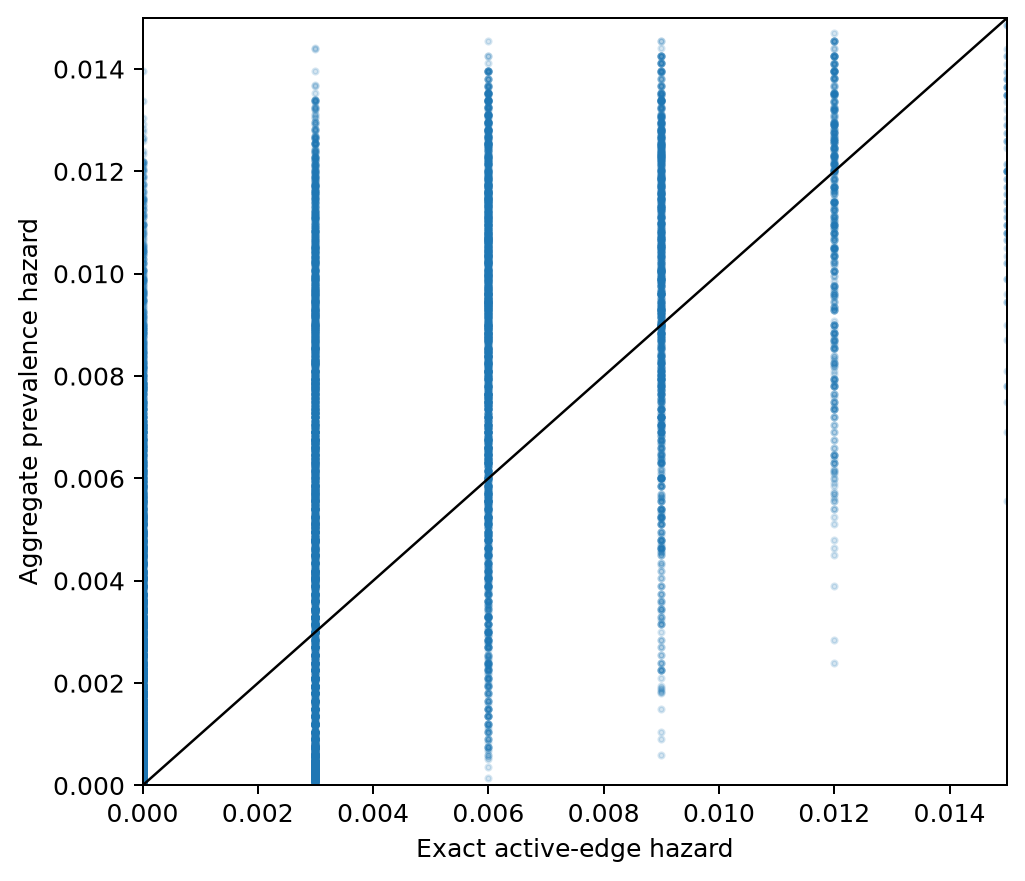
\includegraphics[width=.62\linewidth]{figures/01_exact_vs_aggregate.png}\caption{Exact та aggregate hazards, обчислені на спільних станах Full Micro. Точки є візуалізаційною підвибіркою; inference здійснюється на рівні реплікацій.}\end{figure}
\begin{figure}[H]\centering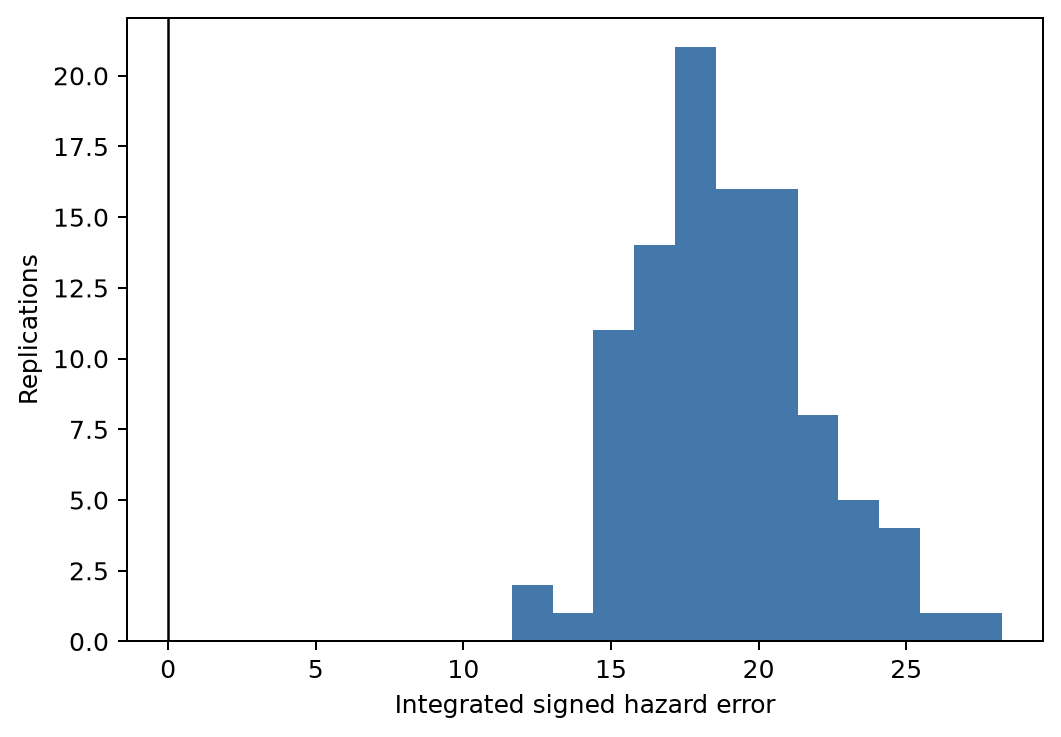
\includegraphics[width=.49\linewidth]{figures/02_signed_error_distribution.png}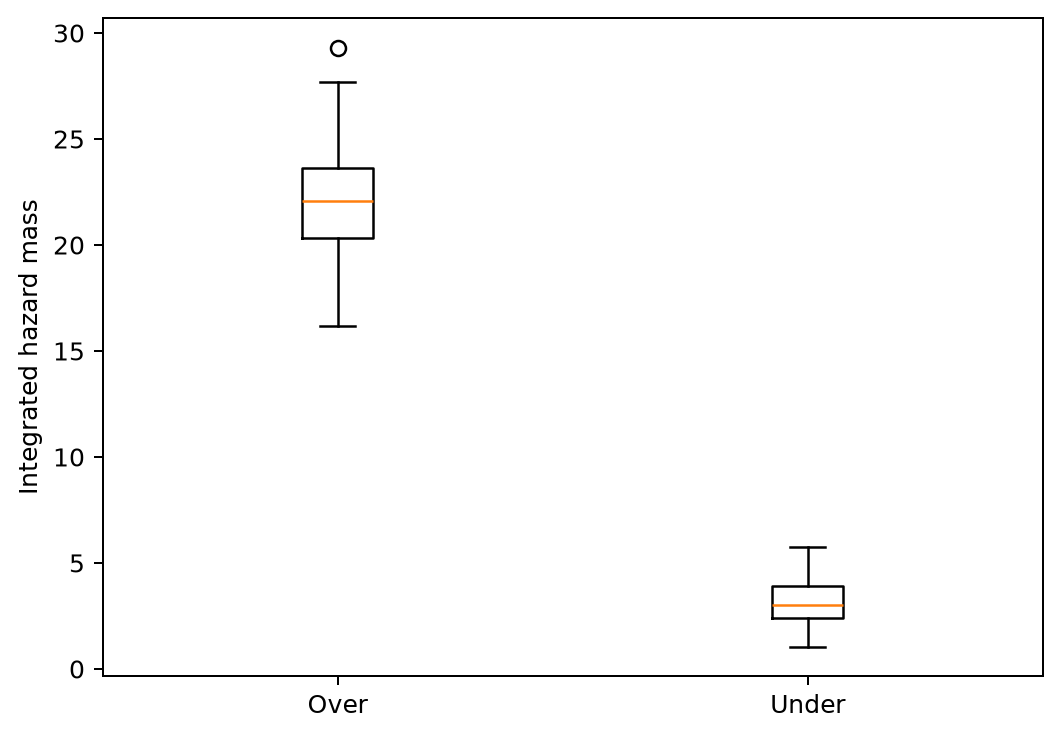
\includegraphics[width=.49\linewidth]{figures/03_over_under_mass.png}\caption{Розподіли за реплікаціями інтегрованої signed error та її over/under компонент.}\end{figure}
\begin{figure}[H]\centering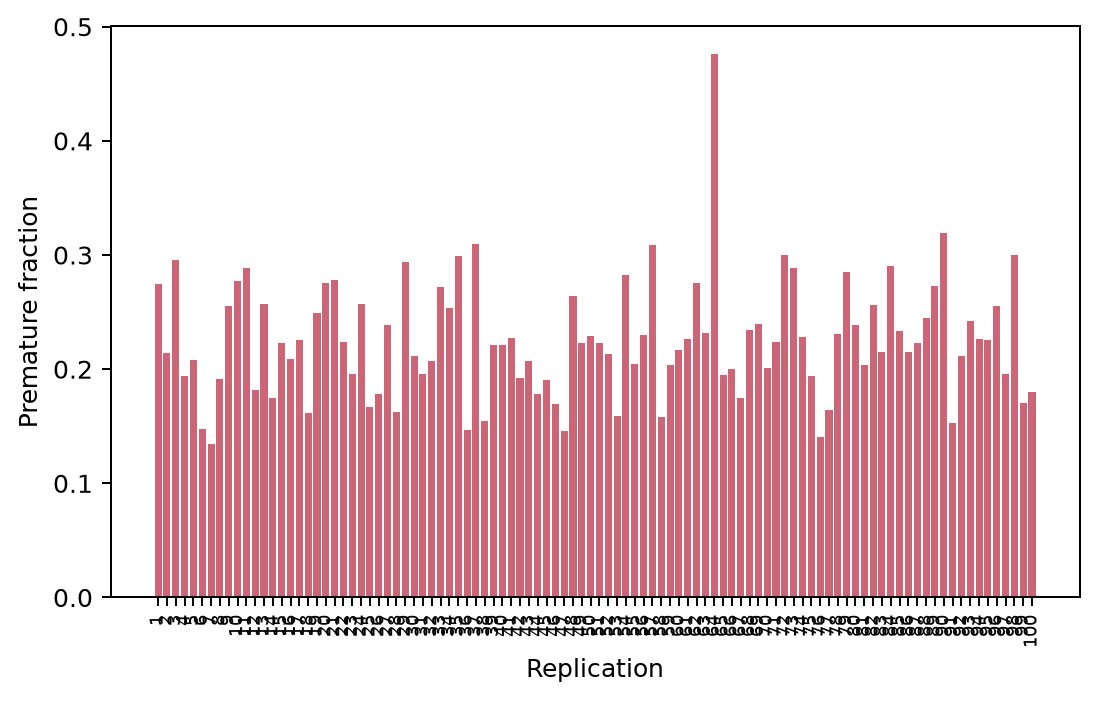
\includegraphics[width=.62\linewidth]{figures/04_premature_fraction.png}\caption{Частка агрегованого cumulative hazard, накопиченого тоді, коли точна inter-community transmission неможлива.}\end{figure}
\begin{figure}[H]\centering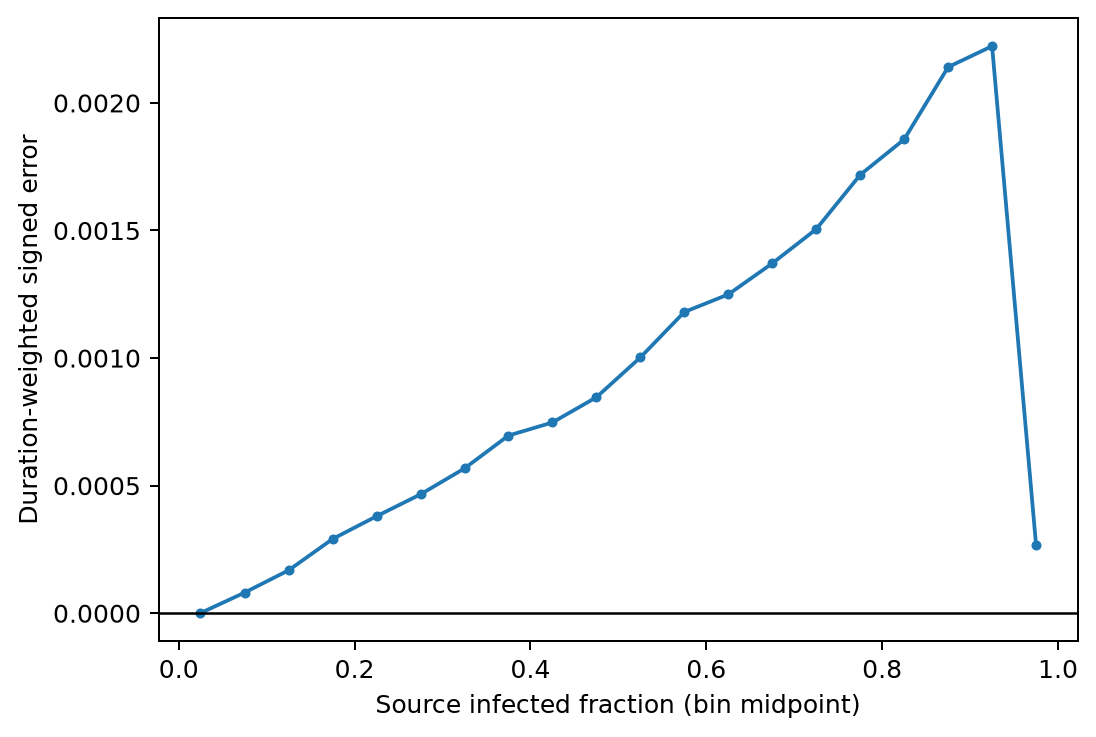
\includegraphics[width=.49\linewidth]{figures/05_error_vs_source_fraction.png}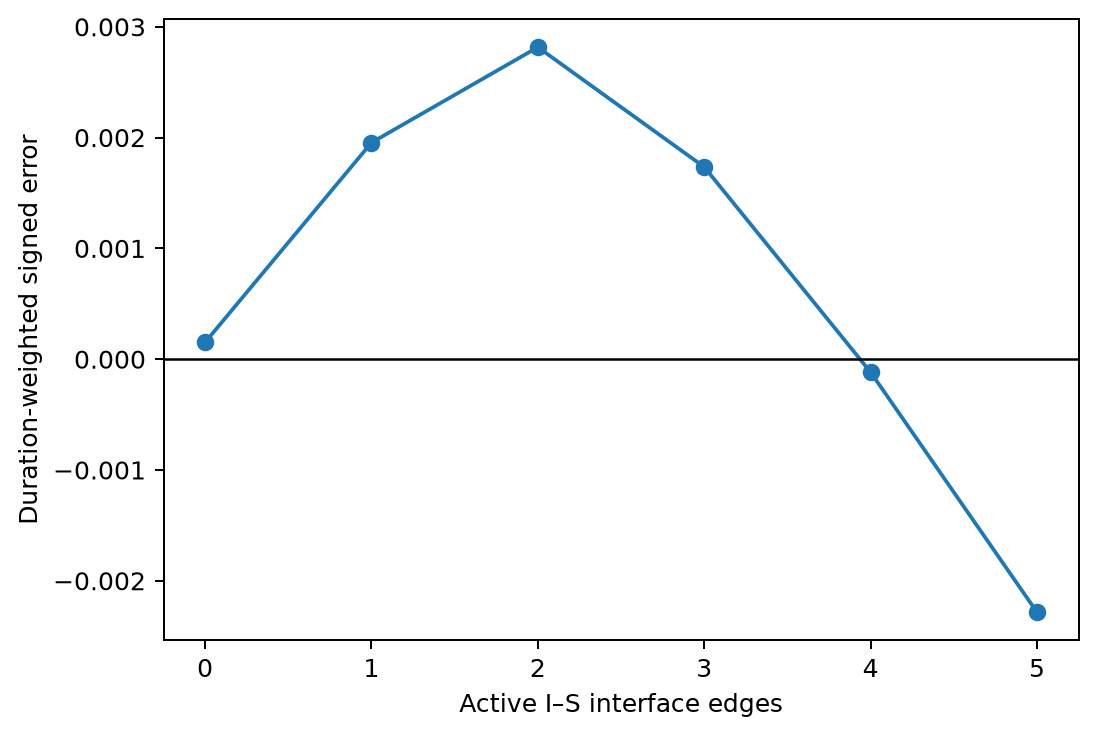
\includegraphics[width=.49\linewidth]{figures/06_error_vs_active_edges.png}\caption{Описова стратифікація на рівні подій. Інтервали є залежними й не трактуються як незалежні спостереження.}\end{figure}
\begin{figure}[H]\centering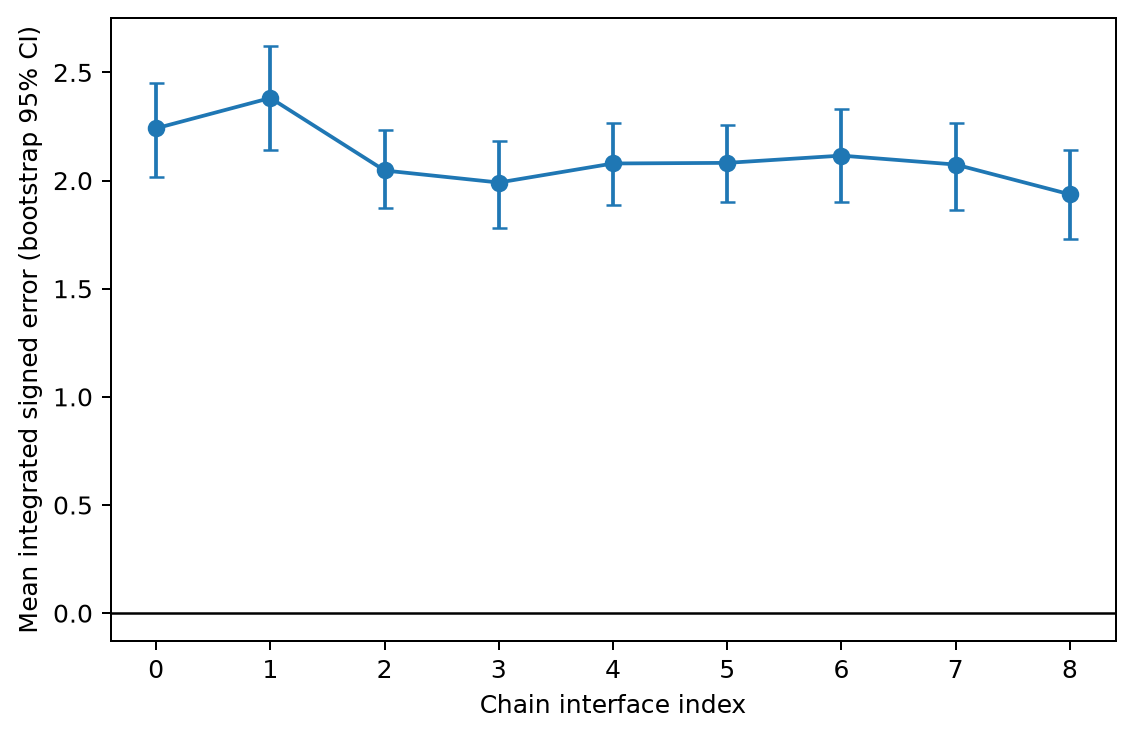
\includegraphics[width=.49\linewidth]{figures/07_layer_integrated_error.png}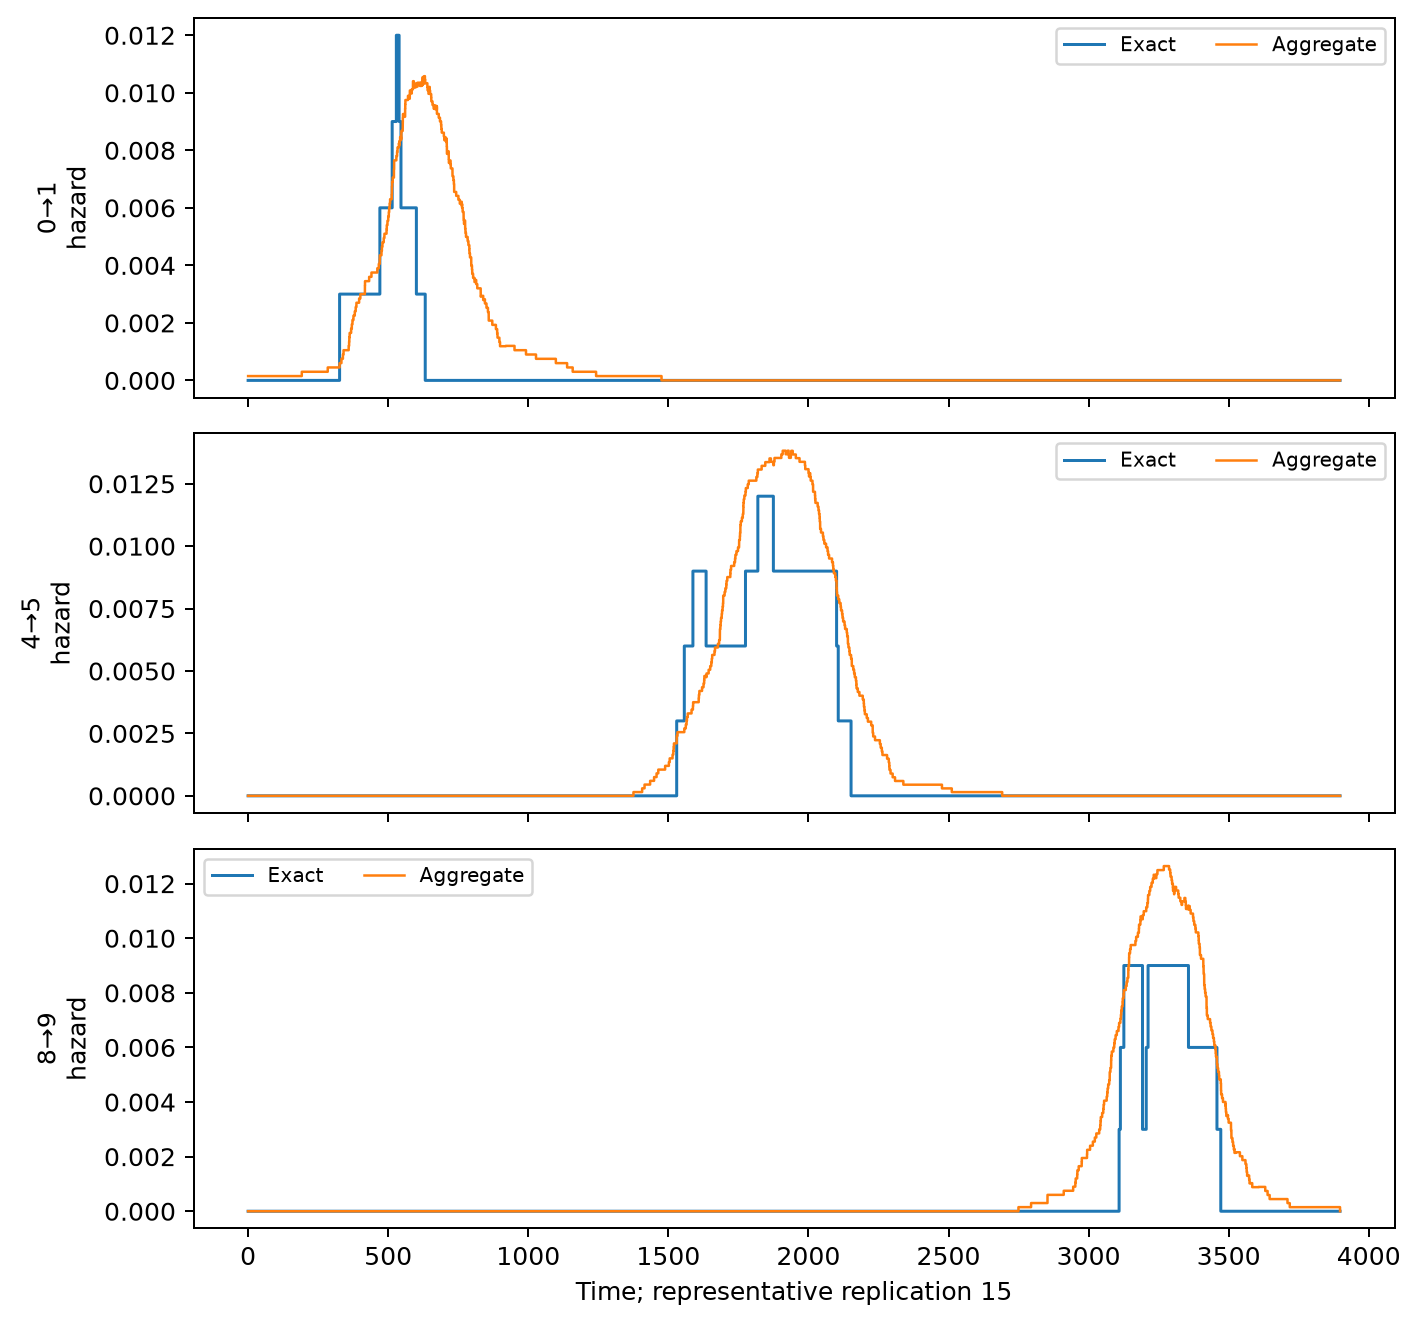
\includegraphics[width=.49\linewidth]{figures/08_representative_time_series.png}\caption{Інтегрована error за layer та репрезентативний часовий ряд спільних станів. Твердження про невизначеність спираються на підсумки реплікацій.}\end{figure}

\section{Наукова інтерпретація}
Signed mass слід інтерпретувати разом з absolute, over-, under- та cumulative premature компонентами: cancellation може зробити signed error малою навіть тоді, коли локальні розбіжності великі. Наведені фінальні оцінки характеризують чисту rate abstraction error на рівні формули для цієї базової конфігурації. Присутні як over-, так і under-hazard mass, хоча середня over-hazard компонента на рівні реплікацій більша для цієї базової конфігурації. Це не встановлює, що агреговані hazards універсально переоцінюють точні hazards.

По реплікаціях середні cumulative exact та aggregate hazards становили 27.131 та 46.078; середні signed та absolute discrepancy masses становили 18.947 та 25.154. Середня over-hazard mass (22.05) перевищувала середню under-hazard mass (3.1035), але ненульова under-компонента підтверджує залежні від стану зміни знаку. Середні 22.537\% агрегованого cumulative hazard накопичувались у станах з нульовим точним active-edge hazard (95\% bootstrap-інтервал 21.56--23.611\%). Стратифіковані за phase середні premature fractions становили 79.201\% early, 30.165\% middle та 20.022\% late. Ці значення за phase описують, де виникає розбіжність формули на replay-траєкторіях; вони не є незалежними оцінками на рівні подій.

\section{Що цей експеримент пояснює --- і чого не пояснює}
Він пояснює розбіжності між двома формулами hazard на спільних станах Full Micro. Він не може пояснити import placement error, продуктивну synchronization error, повну ендогенну trajectory error, зсув event-time лише за signed error чи стійкість до інших топологій або $\gamma>0$.

\section{Обмеження}
Цей фінальний аналіз має 100 реплікацій. Ребра мережі регенерувались, а не архівувались Experiment 01. Кореляції на рівні подій є описовими, оскільки інтервали в межах реплікації залежні. Пороги phase є механістичними фіксованими смугами, а не data-selected changepoints. Узагальнення залишається обмеженим топологією chain та базовою конфігурацією $\gamma=0$.

\section{Рекомендовані наступні експерименти}
Experiment 03 --- це Production vs Event-Driven Synchronization Audit, призначений пояснити відмінність між приблизно 7.5\% error для event-driven aggregate/uniform Experiment 01 та приблизно 42.6\% у продуктивному розрідженому benchmark. Experiment 04 --- це Gateway-Distance Experiment з near/medium/far gateway placement за фіксованих $n,m,d,k,\beta$ та кількості громад. Experiment 04 тут не запускався.

\section{Точні команди для відтворення}
\begin{verbatim}
.venv/bin/python -m unittest tests.test_experiment_02_state_replay_hazard_audit
.venv/bin/python extrascripts/run_experiment_02_state_replay_hazard_audit.py --stage smoke --resume
.venv/bin/python extrascripts/run_experiment_02_state_replay_hazard_audit.py --stage validation --resume
.venv/bin/python extrascripts/analyze_experiment_02_state_replay_hazard_audit.py --stage validation
# Only after explicit approval:
.venv/bin/python extrascripts/run_experiment_02_state_replay_hazard_audit.py --stage final --audit-approved --resume
\end{verbatim}
\end{document}
